
\section{Routing with RPL}

\subsection{Routing Protocols}

There are two classes of routing protocols:
\begin{itemize}
    \item Link-State: Each node knows network topologu and runs a shortest-path 
        algorithm $\to$ powerful but require more resources
    \item Distance-Vector: a node only needs to know which neighbor leads
        to which node.
        \begin{itemize}
            \item Each node maintains for each destination, the minimum distance
                and the neighbor to forward to.
        \end{itemize}
\end{itemize}

\paragraph{Count To Infinity problem with DSV routing}
\begin{figure}[ht!]
    \centering
    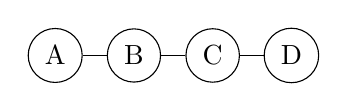
\begin{tikzpicture}
        \node[shape=circle,draw](a){A};
        \node[shape=circle,draw,right of=a](b){B};
        \node[shape=circle,draw,right of=b](c){C};
        \node[shape=circle,draw,right of=c](d){D};

        \draw[-] (a) -- (b);
        \draw[-] (b) -- (c);
        \draw[-] (c) -- (d);
    \end{tikzpicture}
    \caption{Count-To-Infinity, distance metric: number of hops}
\end{figure}

\begin{enumerate}
    \item Initial state: B knows that A is 1 hop away
    \item A disappears. B removes it from its routing table
    \item Before B notifies C, C sends that A is 2 hop away to B
    \item B thinks it has found a new path to A, so it store this path
        and send that A is 3 hop-away
    \item C update its routing table A is 4 hop away and sends
    \item \ldots
\end{enumerate}

\subsection{RPL}

RPL is a routing protocol designed for Low-power and Lossy Networks (LLN).
Characteristics of such networks:

\begin{itemize}
    \item Lossy, slow and unstable links
    \item Traffic mostly flows form devices to a server/sink or border
        router( or in opposite direction)
    \item Large number of nodes
    \item Constrained devices with small memory
\end{itemize}

\subsubsection{Routing Topology}

Topology represented as a Destination Oriented Directed Acyclic Graph (DODAG)
where the root is a server, border router, etc.
\begin{figure}[ht!]
    \centering
    \begin{tikzpicture}
        \node[shape=circle,draw,fill=green](root){0};
        \node[shape=circle,draw,below left of=root](c1){1};
        \node[shape=circle,draw,below right of=root](c2){1};
        \node[shape=circle,draw,below left of=c2](c3){2};
        \node[shape=circle,draw,below right of=c3](c4){3};
        \node[shape=circle,draw,below left of=c3](c5){3};

        \node[left =1cm of root](ds){};
        \node[below =2cm of ds](de){};

        \node[right =1cm of root](us){};
        \node[below =2cm of us](ue){};

        \draw[->] (c1) -- (root);
        \draw[->] (c2) -- (root);
        \draw[->] (c3) -- (c1);
        \draw[->] (c3) -- (c2);
        \draw[->] (c4) -- (c3);
        \draw[->] (c5) -- (c3);
        \draw[->] (c4) -- (c2);
        \draw[->] (c5) -- (c1);

        \draw[->] (ds) -- (de);
        \draw[->] (ue) -- (us);
    \end{tikzpicture}
    \caption{root in green, number correspond to node rank}
\end{figure}
\begin{itemize}
    \item Not a tree as they are multiple path possible for a destination.
    \item An RPL instance is a set disjoint DODAGS
    \item You can have multiple RPL instances on the same physical network
    \item Each RPL control messages carry a DODAG ID and a RPL-instance ID
    \item Rank is node property, typically proportional to path cost but coarser.
        The rank of node must be greater than rank of parent.
\end{itemize}

\subsubsection{RPL Control Messages}
\begin{itemize}
    \item \textbf{DAG Information Object (DIO)}
        \begin{itemize}
            \item Link-local multicasted by existing RPL nodes to advertise a DODAG
            \item Sent periodically by but also on request when routing problem detected
            \item Contains rank od sending node and network prefix
            \item Nodes find parent(s) in this way
            \item Multiple parents possible. Choice depends on path costs
        \end{itemize}
        $\Rightarrow$ Nodes know about possible parents and routes up toward DODAG root
        established.

        \paragraph{Version Number} When the root advertises a DODAG with
        the DIO message, it also includes a version number
        \begin{itemize}
            \item A that joins a DODAG with version X ignores lower versions
            \item When a node receives a message with higher version, it can move to that 
                version $\to$ new rank and parent
        \end{itemize}

        The root can decide to increase the version number and advertise
        a new version of the DODAG. It typically happens when a problem
        with current DODAG is detected and there is a repair.

        \paragraph{Path Cost} To compute how expensive a path is, the
        DODAG can define a Objective Function that the nodes must used.
        Cost can expressed in terms of:
        \begin{itemize}
            \item Signal quality
            \item Throughput
            \item Delay
        \end{itemize}

    \item \textbf{Destination Advertisement Object (DAO)}
        \begin{itemize}
            \item DAO messages travel up and forwarded to root
            \item Are unicasted to parent (or link-local multcasted to help for 
                direct P2P traffic)
            \item The goal is to propagate information about children(new and disappeared)
                so that parents can populate their routing table.
        \end{itemize}
        $\Rightarrow$ Routes down away from root established

    \item \textbf{DODAG Information Solicitation (DIS)}
        Node send DIS message to request DIO when:
        \begin{itemize}
            \item A new node want to joins an RPL instance
            \item A sleeping node wakes up and needs recent information
                about the network or want to inform the network that it is back
            \item A node cannot reach the router anymore $\to$ looking
                for a new parent
        \end{itemize}
\end{itemize}


\subsection{Packet Forwarding}
\begin{itemize}
    \item In up direction $\Rightarrow$ Packet is sent to lower rank (or
        siblings, if no lower rank)
    \item In down direction $\Rightarrow$ Node knows route to
        destination thanks to DAO message
\end{itemize}
Node only store information about next hop to destination, it's a DSV
with ranks.

\subsubsection{Loop Avoidance Mechanism}

\begin{itemize}
    \item \textbf{IPv6 header option}

        There is a direction flag in the header indicating the expected direction
        of a data packet:
        \begin{itemize}
            \item Sender sets the direction
            \item If an up-packet is forwarded from a node A to a node B with 
                higher rank, a problem is detected by B (same in opposed situation)
            \item Node B sets the R (repair flag) in the packet. This indicates
                that the DODAG has to be repaired
        \end{itemize}

    \item \textbf{Node movement}
        Node might find better parents:
        \begin{itemize}
            \item New nodes appear or old nodes disappear
            \item Signal strength changes
        \end{itemize}
        However, node are only allowed to move up toward the root $\Rightarrow$ A node
        cannot become a child of one of its children.
\end{itemize}

\subsubsection{Trickle Timer}
A DIO message are sent to build new DODAG, on a DIS message and
periodically. To avoid that to send to many DIO when it's not necessary,
a Trikle Timer is run on each node:

\begin{itemize}
    \item $T_min$: minimum duration of the timer
    \item $T_max$: maximum duration of the timer
    \item $T$: current duration used by the timer
    \item $C$: number of good messages received by the node
    \item $K$: some threshold for C
\end{itemize}

\begin{small}
    \begin{lstlisting}[frame=single]
    T:= Tmin, C:=0
    t = rand(T/2,T)
    wait(event)

    if event == t expires and C<K:
        send DIO 
        restart t

    if event == T expires:
        T:= 2*T (up to Tmax)
        restart T

    if event == good DIO:
        C:= C+1
    if event == bad DIO:
        C:= 0
        T= Tmin
    \end{lstlisting}
\end{small}

\begin{itemize}
    \item C is increased by 1 for every good message = DIO that does not announce a
        change
    \item C is reset to 0 and T is reset to $T_min$ for bad message= DIO that 
        announces a change or with R flag.
\end{itemize}
Good message indicate a stable network and because T is increased,
nodes send DIS messages less messages less frequently.


